\documentclass[oneside]{caesar_book}

%%%%%%%%%%%%%%%%%%%    PACKAGES    %%%%%%%%%%%%%%%%%%%
%% Font
\usepackage{fontspec}
	\setmainfont{TexGyrePagella}

\usepackage{fontawesome5}

\usepackage{unicode-math}
	\setmathfont{TexGyrePagella-math}

%% Languages
\usepackage{polyglossia}
	\setdefaultlanguage[variant=british]{english}

%% Author affiliation
\usepackage{authblk}

%% Figures...
% ...graphics
\usepackage[luatex]{graphicx}

\usepackage[font = small]{caption}
\usepackage{subcaption}
	\captionsetup{subrefformat=parens}
	% \captionsetup[subfigure]{skip=-30pt} % aboveskip=-30pt,belowskip=-2pt,

% ...Colours
\usepackage{xcolor}
	\definecolor{egyptRed}{HTML}{DD5129}
	\definecolor{egyptBlue}{HTML}{0F7BA2}
	\definecolor{egyptGreen}{HTML}{43B284}
	\definecolor{egyptYellow}{HTML}{FAB255}
	\definecolor{lightGrey}{HTML}{CCCCCC}

% ...TikZ coding
\usepackage{tikz}
	\usetikzlibrary{arrows.meta}
	\tikzset{arrow/.style = {> = {Latex[length = 1.2mm]}}}
	\usetikzlibrary{positioning}
	\usetikzlibrary{calc}
	\usetikzlibrary{fit}
	\usetikzlibrary{backgrounds} % Can be useful for debugging, i.e. check the frame of a tikz picutre. For this \begin{tikzpicture}[framed]

% Define database node
\makeatletter
	\tikzset{
		database/.style={
			path picture={
			\draw[fill = egyptYellow] (0, 1.5*\database@segmentheight) circle [x radius=\database@radius,
			y radius=\database@aspectratio*\database@radius];
			\draw (-\database@radius, 0.5*\database@segmentheight) arc [start angle=180,end angle=360,x radius=\database@radius,
			y radius=\database@aspectratio*\database@radius];
			\draw (-\database@radius,-0.5*\database@segmentheight) arc [start angle=180,end angle=360,x radius=\database@radius,
			y radius=\database@aspectratio*\database@radius];
			\draw (-\database@radius,1.5*\database@segmentheight) -- ++(0,-3*\database@segmentheight) arc [start angle=180,end angle=360,
			x radius=\database@radius, y radius=\database@aspectratio*\database@radius] -- ++(0,3*\database@segmentheight);
			},
			minimum width=2*\database@radius + \pgflinewidth,
			minimum height=3*\database@segmentheight + 2*\database@aspectratio*\database@radius + \pgflinewidth,
		},
		database segment height/.store in=\database@segmentheight,
		database radius/.store in=\database@radius,
		database aspect ratio/.store in=\database@aspectratio,
		database segment height=0.1cm,
		database radius=0.25cm,
		database aspect ratio=0.35,
	}
\makeatother

%% Links
\usepackage{url}
\usepackage[luatex, colorlinks=true, linkcolor=egyptBlue, urlcolor=egyptRed, citecolor=egyptGreen]{hyperref}

%% Bibliography
\usepackage{csquotes}
\usepackage[backend=biber,style=philosophy-classic]{biblatex}
\addbibresource{./centralised_bibliography/references.bib}

%% Mathematics
\usepackage{amsmath}
\usepackage{siunitx}
\usepackage{xfrac}

%% Tables
\usepackage{booktabs}

%% Info box
\usepackage[most]{tcolorbox}
% \newtcolorbox{infobox}{}{%

% }%

% Information about the book
% to be put on the title page
\title{Technical note on total and bole volumes, and on wood density to the Conseil Scientifique et Technique de l'IGN}

\author{Amaël Le Squin, Florence Gohon, Henri Cuny}

\publisher{}

%----------------------------------------------------------------------------------------
%	NEW COMMANDS
%----------------------------------------------------------------------------------------

%% Text
\newcommand{\EFM}{EFM}
\newcommand{\NFI}{NFI}
\newcommand{\ie}{\textit{i.e., }}
\newcommand{\eg}{\textit{e.g., }}

%% Maths
% Shortcuts
\newcommand{\Vtot}{V_{\text{tot}}}
\newcommand{\Vbole}{V_{\text{bole}}}
\newcommand{\Sigmabf}{\symbfup{\Sigma}}

% Operators
\DeclareMathOperator{\logit}{logit}
\DeclareMathOperator{\MVN}{MVN}
\DeclareMathOperator{\Cov}{Cov}
\DeclareMathOperator{\E}{\mathbb{E}}

\begin{document}
% no page numbering in front matter
\frontmatter
% generate the title page
\maketitlepage
% show the table of contents
\tableofcontents
% start to number the pages
\mainmatter

\chapter{Context\label{chap::context}}

The French National Forest Inventory (\NFI) publishes statistics annually, such as basal area or wood resources, on both private and public forest. These statistics are derived from a sampling scheme in which about \num{6000} new plots are surveyed each year, along with \num{6000} plots that were first visited five years earlier. The published statistics are calculated using a moving five-year average; for instance, the published results for 2024 are based on campaigns spanning from 2020 to 2024. \\

Initially designed to assess forest area and produce estimates of standing timber stock, the French \NFI{} is gradually evolving into more comprehensive tools for forest monitoring, incorporating a variety of indicators. Among this new information, the estimation of forest biomass and carbon is crucial, as it makes it possible to monitor biomass production and its use by different sectors, to estimate the contribution of forests to mitigating the effects of climate change as part of climate commitments monitoring (Citepa), and to develop forest strategies adapted to contemporary environmental and societal challenges \parencite{Commission2018}. \\

% Check \sidecite, and maybe tweak it to put only the author and title in the margin

The European Union developed a \href{https://eur-lex.europa.eu/legal-content/EN/TXT/?uri=CELEX:52021DC0572}{New EU Forest Strategy for 2030} as part of the plan to adapt to and fight against climate change and make Europe a climate neutral continent by 2050. This strategy relies on improved monitoring of European forests to better understand their condition and respond accordingly. Specifically, it calls for assessing carbon sequestration in forests to evaluate whether or not Eu\-ro\-pe reached carbon neutrality. One bottleneck is the harmonisation of the forest monitoring methods between European member states, if not within them. The \href{https://pathfinder-heu.eu/#top}{PathFinder project} supports member states in implementing a European Forest Monitoring System in order to standardise or harmonise forest data collection and reporting across the EU. This prompted the French \NFI{} to update its methods for assessing forest carbon storage. \\

Three steps are necessary to estimate carbon storage from field data (see Fig. \ref{fig::scheme}): (\textit{i}) the total aerial volume is estimated from diameter at breast height (dbh) and height \parencite{Vallet2006}, (\textit{ii}) biomass is then derived by using a coefficient for wood density, and (\textit{iii}) a factor is applied to convert the biomass into carbon content. \\

\begin{figure}[h]
    \centering
	\begin{tikzpicture}
	\node (vol) at (0, 0) {Volume};
	\node[below = of vol.mid east, anchor = mid east] (dens) {Density};

	\path (vol.mid east) -- (dens.mid east) node[midway, right = 0.8cm, anchor = mid west] (bio) {Biomass};
	\draw[->, arrow, out = 0, in = 180] (vol.mid east) to (bio.mid west);
	\draw[->, arrow, out = 0, in = 180] (dens.mid east) to (bio.mid west);

	\node[right = 0.8cm of bio.mid east, anchor = mid west] (C) {Carbon};
	\draw[->, arrow] (bio.mid east) to (C.mid west);

	\node[database, above left = 0.3cm of vol, label = above:Emerge, database radius = 0.3cm,
		database segment height = 0.15cm] (emerge) {};

	\node[database, below left = 0.3cm of dens, label = below:XyloDensMap, database radius = 0.3cm,
		database segment height = 0.15cm] (xdm) {};

	\draw[->, arrow, dashed, out = -90, in = 180] (emerge.south) to (vol.mid west);
	\draw[->, arrow, dashed, out = 90, in = 180] (xdm.north) to (dens.mid west);
\end{tikzpicture}
	\caption{Computation chain for biomass and carbon content.\label{fig::scheme}}
\end{figure}

In this technical note, we explain the methods we foresee to estimate the two volumes computed at the French \NFI{} for each tree: the bole volume (volume bois-fort tige), which is the reference volume since the creation of the French \NFI{} (1958), and the total aerial volume. In the section \nameref{chap::def}, we define the different tree components and explain the origins of the data. Then, in the section \nameref{chap::bole_v}, we expose the method to compute the individual bole volume, and lastly we describe the model for total volume in the section \nameref{chap::total_v}.

\chapter{Definitions and datasets\label{chap::def}}

Trees are partitioned into hierarchical elements with definitions that may vary between Forest Inventories and datasets (\eg Fig. \ref{fig::partition}).

\begin{figure*}[h]
	\centering
	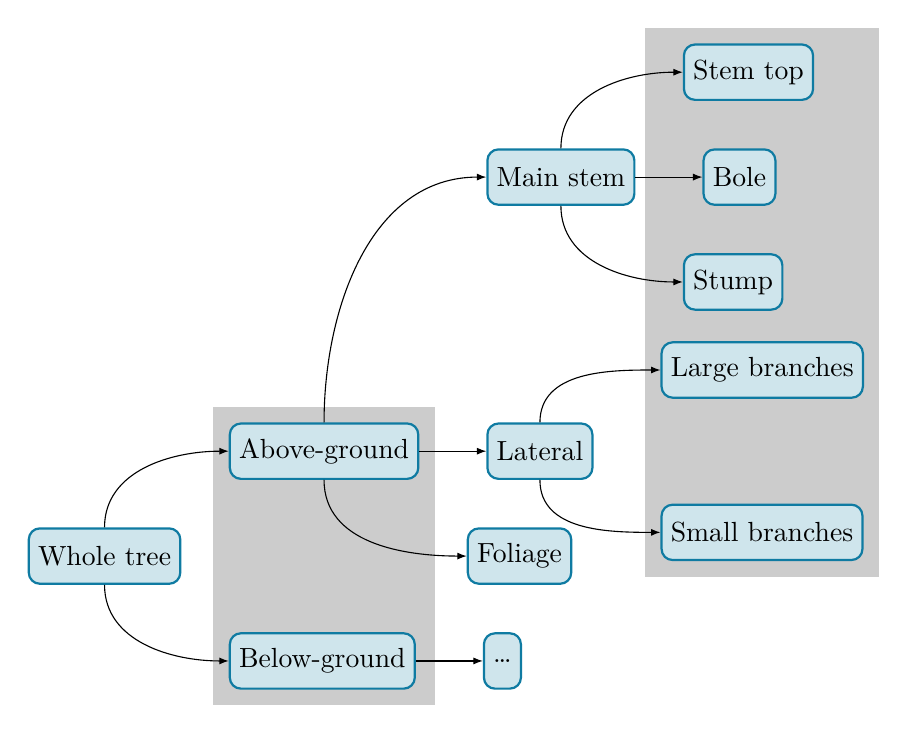
\begin{tikzpicture}[block/.style = {rectangle, draw = egyptBlue, thick, fill = egyptBlue!20, rounded corners, minimum height = 2em}]
	%% Level 0
	\node[block] (orig) at (0, 0) {Whole tree};
	
	%% Level 1
	\node[block, above right = 0.85cm of orig] (aboveground) {Above-ground};
	\node[block, below right = 0.85cm of orig] (belowground) {Below-ground};

	\begin{scope}[on background layer] % From background library
		\node[fit=(belowground)(aboveground), fill = lightGrey, inner sep=2mm] {};
	\end{scope}
	
	%% Level 2
	\node[block, above right = 2.75cm and 0.85cm of aboveground] (stem) {Main stem};
	\node[block, right = 0.85cm of aboveground] (lat) {Lateral};
	\node[block, below right = 0.85cm of aboveground] (fol) {Foliage};
	
	\node[block, right = 0.85cm of belowground] (root) {\dots};

	%% Level 3
	\node[block, above right = 0.85cm of stem] (stemtop) {Stem top};
	\node[block, right = 0.85cm of stem] (bole) {Bole};
	\node[block, below right = 0.85cm of stem] (stump) {Stump};

	\node[block, draw, above right = 0.3cm and 0.85cm of lat] (lbranch) {Large branches};
	\node[block, draw, below right = 0.3cm and 0.85cm of lat] (sbranch) {Small branches};
	
	\begin{scope}[on background layer] % From background library
		\node[fit=(sbranch)(stemtop), fill = lightGrey, inner sep=2mm] {};
	\end{scope}

	%% Arrows...
	% ... 0 to 1
	\draw[->, arrow] (orig.north) to[out = 90, in = 180] (aboveground.west);
	\draw[->, arrow] (orig.south) to[out = -90, in = 180] (belowground.west);

	% ... 1 to 2
	\draw[->, arrow] (aboveground.north) to[out = 90, in = 180] (stem.west);
	\draw[->, arrow] (aboveground.east) -- (lat.west);
	\draw[->, arrow] (aboveground.south) to[out = -90, in = 180] (fol.west);
	
	\draw[->, arrow] (belowground.east) -- (root.west);

	% ... 2 to 3
	\draw[->, arrow] (stem.north) to[out = 90, in = 180] (stemtop.west);
	\draw[->, arrow] (stem) -- (bole.west);
	\draw[->, arrow] (stem.south) to[out = -90, in = 180] (stump.west);

	\draw[->, arrow] (lat.north) to[out = 90, in = 180] (lbranch.west);
	\draw[->, arrow] (lat.south) to[out = -90, in = 180] (sbranch.west);
\end{tikzpicture}
	\caption{Hierarchical elements of trees, figure inspired by \cite{Gschwantner2009} \label{fig::partition}}
\end{figure*}

In our case, the tree data come from different institutes, different periods of time, and do not all have the same tree components recorded:

\begin{marginfigure}%
	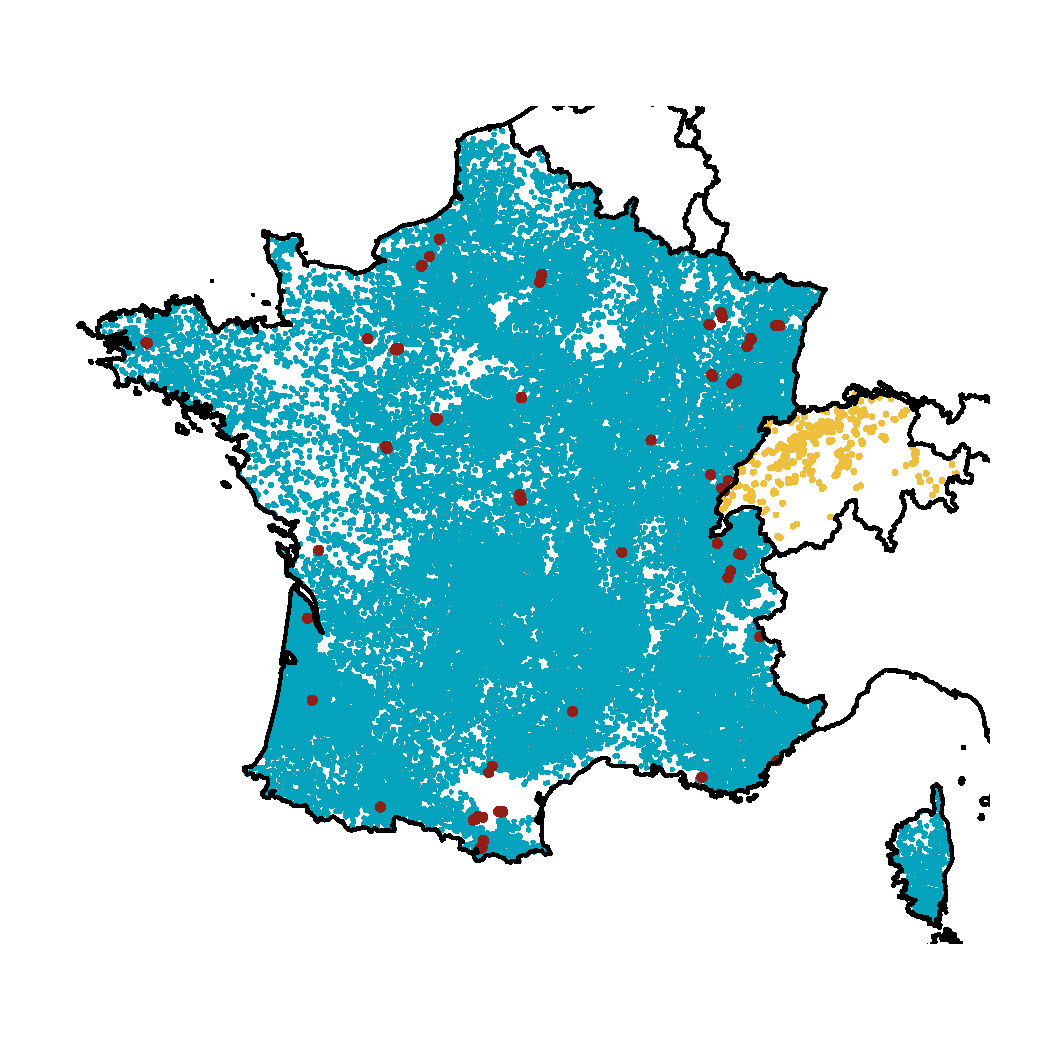
\includegraphics[width=\marginparwidth]{./Figures/map.png}
	\caption{Plot location for French \NFI, Emerge, and Swiss dataset.\label{fig::map}}
\end{marginfigure}

\begin{enumerate}
	\item `Protocole Oudin', dataset preserved by INRAE, ranging from 1930 to 1980 (in red on Fig. \ref{fig::map}). Recorded the bole volume, and the large and small branches. Hereafter, we name this dataset `Emerge', which was the name of the project that digitalised this dataset in 2008 \parencite{Deleuze2013}.
	\item The French \NFI (in blue on the Fig. \ref{fig::map}). Data range from 1988 to 2007 (data before 1988 record diameter rather than circumference). Recorded the bole volume.
	\item Experimental Forest Management project dataset \parencite[in yello on Fig. \ref{fig::map}]{Didion2024}. Data range from 1888 to 1974, and bole volume, large branches, and small branches were recorded.
	\item The `Office National des Forêts (ONF)', with protocols from 1972 and from 1983 (not used as there is no coordinates)
	\item Institut Technologique Forêt, Cellulose, Bois-construction, Ameublement (FCBA), not used so far for the aerial volume
	\item L'Institut pour le développement forestier (IDF) which is the R\&D of the Centre National de la Propriété Forestière and the Institut national de recherche en sciences et technologies pour l'environnement et l'agriculture (IRSTEA, currently INRAE)
\end{enumerate}

We decided to use the definitions from \cite{Gschwantner2009} (see Figs. \ref{fig::partition} and \ref{fig::ign_tree}):

\begin{marginfigure}%
	\begin{tikzpicture}
	\node (tree) at (0, 0) {\includegraphics[width=\marginparwidth]{./Figures/ign_tree.pdf}};
	\matrix[below = -0.2cm of tree] {
		\node [draw, shape = rectangle, fill = egyptYellow, label = right:Bole] {}; \\
		\node [draw, shape = rectangle, fill = egyptGreen, label = right:Large branches] {}; \\
		\node [draw, shape = rectangle, fill = egyptBlue, label = right:Small branches] {}; \\
	};
\end{tikzpicture}
	\caption{Scheme of tree components.\label{fig::ign_tree}}
\end{marginfigure}

\begin{itemize}
	\item Main stem: The stem of a tree is the above-ground part of the main (off) shoot with apical dominance
	\begin{itemize}
		\item Stem top: topmost part of the stem from an over-bark base-diameter of \qty{7}{\centi\metre} (French \NFI) to the stem tip
		\item Bole: above-ground part of the stem between stump and the stem top
		\item Stump: above-ground base part of the stem which would remain after a tree was cut under normal felling practices
	\end{itemize}
	\item Lateral parts:
	\begin{itemize}
		\item Large branches: portion of the above-ground lateral parts with a diameter of more than or equal to \qty{7}{\centi\metre} (French \NFI)
		\item Large branches: portion of the above-ground lateral parts with a diameter of less than \qty{7}{\centi\metre} (French \NFI)
	\end{itemize}
\end{itemize}

A total of \num{594616} individuals were measured, with 98\% coming from the \NFI{} (bole volume only), 6\% from the Swiss dataset (bole, large and small branches), and 2\% from Emerge (same components as the Swiss dataset; see Fig. \ref{fig::compo}). The difficulties in fitting the data are twofold: first, the data show high heteroskedasticity (see Fig \ref{fig::fagSyl}), and second, the datasets are unbalanced.

\begin{figure}
	\centering
	% Created by tikzDevice version 0.12.6 on 2025-10-06 15:09:30
% !TEX encoding = UTF-8 Unicode
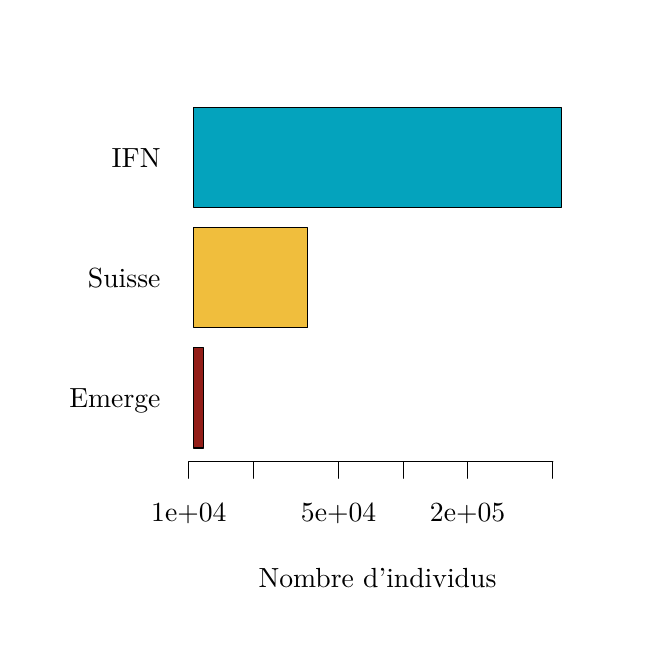
\begin{tikzpicture}[x=1pt,y=1pt]
\definecolor{fillColor}{RGB}{255,255,255}
\path[use as bounding box,fill=fillColor,fill opacity=0.00] (0,0) rectangle (216.81,216.81);
\begin{scope}
\path[clip] (  0.00,  0.00) rectangle (216.81,216.81);
\definecolor{drawColor}{RGB}{0,0,0}
\definecolor{fillColor}{RGB}{147,30,24}

\path[draw=drawColor,line width= 0.4pt,line join=round,line cap=round,fill=fillColor] ( 60.00, 64.92) rectangle ( 63.54,101.09);
\definecolor{fillColor}{RGB}{240,190,61}

\path[draw=drawColor,line width= 0.4pt,line join=round,line cap=round,fill=fillColor] ( 60.00,108.32) rectangle (101.25,144.49);
\definecolor{fillColor}{RGB}{4,163,189}

\path[draw=drawColor,line width= 0.4pt,line join=round,line cap=round,fill=fillColor] ( 60.00,151.72) rectangle (192.81,187.89);
\end{scope}
\begin{scope}
\path[clip] (  0.00,  0.00) rectangle (216.81,216.81);
\definecolor{drawColor}{RGB}{0,0,0}

\node[text=drawColor,anchor=base east,inner sep=0pt, outer sep=0pt, scale=  1.00] at ( 48.00, 79.56) {Emerge};

\node[text=drawColor,anchor=base east,inner sep=0pt, outer sep=0pt, scale=  1.00] at ( 48.00,122.96) {Suisse};

\node[text=drawColor,anchor=base east,inner sep=0pt, outer sep=0pt, scale=  1.00] at ( 48.00,166.36) {IFN};
\end{scope}
\begin{scope}
\path[clip] (  0.00,  0.00) rectangle (216.81,216.81);
\definecolor{drawColor}{RGB}{0,0,0}

\node[text=drawColor,anchor=base,inner sep=0pt, outer sep=0pt, scale=  1.00] at (126.41, 14.40) {Nombre d'individus};
\end{scope}
\begin{scope}
\path[clip] (  0.00,  0.00) rectangle (216.81,216.81);
\definecolor{drawColor}{RGB}{0,0,0}

\path[draw=drawColor,line width= 0.4pt,line join=round,line cap=round] ( 58.25, 60.00) -- (189.79, 60.00);

\path[draw=drawColor,line width= 0.4pt,line join=round,line cap=round] ( 58.25, 60.00) -- ( 58.25, 54.00);

\path[draw=drawColor,line width= 0.4pt,line join=round,line cap=round] ( 81.56, 60.00) -- ( 81.56, 54.00);

\path[draw=drawColor,line width= 0.4pt,line join=round,line cap=round] (112.37, 60.00) -- (112.37, 54.00);

\path[draw=drawColor,line width= 0.4pt,line join=round,line cap=round] (135.67, 60.00) -- (135.67, 54.00);

\path[draw=drawColor,line width= 0.4pt,line join=round,line cap=round] (158.98, 60.00) -- (158.98, 54.00);

\path[draw=drawColor,line width= 0.4pt,line join=round,line cap=round] (189.79, 60.00) -- (189.79, 54.00);

\node[text=drawColor,anchor=base,inner sep=0pt, outer sep=0pt, scale=  1.00] at ( 58.25, 38.40) {1e+04};

\node[text=drawColor,anchor=base,inner sep=0pt, outer sep=0pt, scale=  1.00] at (112.37, 38.40) {5e+04};

\node[text=drawColor,anchor=base,inner sep=0pt, outer sep=0pt, scale=  1.00] at (158.98, 38.40) {2e+05};
\end{scope}
\end{tikzpicture}

	\caption{Composition of the used dataset for the bole volume and total aerial volume.\label{fig::compo}}
\end{figure}

\begin{figure}
	\centering
	\includegraphics[scale = 0.5]{Figures/resp_fagus.pdf}
	\caption{Typical response of bole volume to circumference (here displayed for \textit{Fagus sylvatica}). We can see that both the Emerge and Swiss datasets \parencite{Deleuze2013,Didion2024} are quite similar and covers elongated trees, while the French \NFI{} covers less regular trees. \label{fig::fagSyl}}
\end{figure}

\begin{tcolorbox}[breakable, title = Bole volume (volume bois-fort tige)]
	The bole volume is the `reference' volume since the creation of the French \NFI{} (1958). Its definition is largely driven by the requirements of the wood industry, for which the estimation of standing timber volume is an essential tool for resource management and planning.
\end{tcolorbox}
\chapter{Bole volume\label{chap::bole_v}}


\chapter{Total above-ground volume\label{chap::total_v}}

In this section, I explore two possible paths to estimate the total above-ground volume, \( \Vtot \). The first option, based on \cite{Longuetaud2013}, uses the ratio:
\begin{equation}
	r = \frac{\Vbole}{\Vtot} \label{eq::r_boletot}
\end{equation}
and is comprised between 0 and 1 by construction. The second option is to fit a multivariate normal distribution, \( \MVN \), to the \textit{transformed} ratio, \( \logit(r) \), jointly with the log-transformed total volume, \( \log(\Vtot) \):
\begin{equation}
	\begin{pmatrix}
		\logit(r) \\
		\log(\Vtot)
	\end{pmatrix}
	\sim
	\MVN\left\{ \begin{pmatrix}
		f(c, \, h; \symbfup{\theta}) \\
		g(c, \, h; \symbfup{\theta}) \\
	\end{pmatrix}, \Sigmabf \right\},
	\label{eq::mvn}
\end{equation}
where \( f \) and \( g \) are functions tailored to our specific needs, \( c \) is circumference at breast height, \( h \), is tree height, and \( \theta \) is a vector of parameters to estimate.

\section{Ratio approach}

I modelled the ratio \( r \) (see equation \eqref{eq::r_boletot}), which quantifies the percentage of volume represented by the bole, by a Beta-distribution. This distribution respects the bounds and accounts for heteroskedasticity, but its parameters \( \text{shape}_1 \) and \( \text{shape}_2 \) are not intuitive. Hence, I reparametrised the Beta-distribution in function of its mean, \( \mu \) and precision, \( \phi \):
\begin{align*}
	\text{shape}_1 &= \phi \mu \\
	\text{shape}_2 &= \phi (1 - \mu)
\end{align*}

Employing the mean and variance is not advisable, since it introduces the interacting constraint \( \sigma^2 < \mu (1 - \mu) \), while the precision lies between 0 and \( + \infty \). The ratio approach has been tested on the 17\textup{th} most common species in the Emerge dataset. The mean \( \mu \) is a function of three parameters to estimate (see equation \eqref{eq::mu-ratio}) and \( \Vbole \), the \textit{predictive variable}:
\begin{equation}
	\mu(\Vbole; \alpha, \beta, \gamma) = \exp[-\beta \Vbole] (\Vbole - \alpha) + \gamma \Vbole + \alpha,
	\label{eq::mu-ratio}
\end{equation}
where \( \alpha, \, \beta\) and \( \gamma \) are parameters to estimate. The results are displayed for \textit{Abies alba} and \textit{Fagus sylvatica}, to represent both conifers and broadleaves (see Fig. \ref{fig::res-mu-ratio}).

\begin{figure}[htb]
	\centering
	\setkeys{Gin}{width=\linewidth}
	\begin{subfigure}{0.4\textwidth}
		\includegraphics{./Figures/abiesAlba.png}
		\caption{\textit{Abies alba}}
	\end{subfigure}
	\hfil
	\begin{subfigure}{0.4\textwidth}
		\includegraphics{./Figures/fagSyl.png}
		\caption{\textit{Fagus sylvatica}}
	\end{subfigure}
	\caption{Fit of the ratio data from Emerge only (circles). The dots are posterior predictions, which are in the range of the observations, although residuals show under-dispersion for small values of \( \Vbole \) (see appendix \ref{app::residuals}). The red curve is the fitted equation \eqref{eq::mu-ratio}}
	\label{fig::res-mu-ratio}
\end{figure}

The equation \eqref{eq::mu-ratio} gives similar predictions (see \ref{fig::pred-ratio}) to \cite{Vallet2006} (currently in use at the \NFI) or Emerge\sidenote{In addition to digitising the dataset related to the `Protocole Oudin', the Emerge project aimed to develop a unified allometry for all tree species in French forests. They arrived at the allometry \[ \Vtot = \frac{c^2 h}{4 \pi (1 - \sfrac{1.3}{h})} \left( \alpha + \beta \frac{\sqrt{c}}{h} + \gamma \frac{h}{c} \right).\]This allometry is not used officially by the French \NFI} \parencite{Deleuze2014}. Responses for the non-displayed species are similar to \textit{Abies alba} and \textit{Fagus sylvatica} results.
\begin{figure}[h]
	\centering
	\setkeys{Gin}{width=\linewidth}
	\begin{subfigure}{0.4\textwidth}
		\includegraphics{./Figures/abiesAlba-pred.png}
		\caption{\textit{Abies alba}}
	\end{subfigure}
	\hfil
	\begin{subfigure}{0.4\textwidth}
		\includegraphics{./Figures/fagSyl-pred.png}
		\caption{\textit{Fagus sylvatica}}
	\end{subfigure}
	\caption{Predictions of total aerial volume in function of bole volume (the explanatory variable) with my model (equation \eqref{eq::mu-ratio}), the current model used at the French \NFI \parencite{Vallet2006}, and the allometry developed during the project Emerge.}
	\label{fig::pred-ratio}
\end{figure}

\section{Multivariate approach}

Multivariate models allow pulling information across components, \ie they describe the variation within and covariation among tree components. I chose to model jointly \( r \) and \( \Vtot \) but the alternative modelling bole and crown could also be considered.

\begin{tcolorbox}[breakable, title = Intractability]
Note that whatever I try to model, there will always be intractability somewhere. If I model both components -- trunk and crown -- with a multivariate lognormal, the distribution of the total volume becomes untractable (sum of two lognormals has no closed form distribution). Alternatively, if I model the total volume and the ratio \( r \), then \( \Vbole \) becomes untractable. Indeed:
\begin{align*}
	\E[\Vbole] &= \E[r \Vtot] \\
	\E[\Vbole] &= \E[r] \E[\Vtot] + \Cov[r, \Vtot]
\end{align*}
and similarly for the variance. In any case, I do not have a closed-form distribution.
\end{tcolorbox}

\subsection{Simulated data}
In order to demonstrate the relevance of multivariate methods, I simulate two correlated random variables and then recover the generating parameters. Let \( X \) be an explanatory variable, and \( \mathbf{Y} = (Y_1, \, Y_2) \) be the dependant variable, such that:
\[
	\begin{pmatrix}
		Y_1 \\
		Y_2
	\end{pmatrix} \sim
	\MVN\left\{ \begin{pmatrix}
		\alpha_1 + \beta_1 X \\
		\alpha_2 + \beta_2 X \\
	\end{pmatrix}, \Sigmabf \right\},
\]
where \( \alpha \) and \( \beta \) are regression parameters to estimate, and \( \Sigmabf \) is the variance-covariance matrix defined by:
\[
	\Sigmabf = \begin{bmatrix}
		\sigma_1^2 & \rho \sigma_1 \sigma_2 \\
		\rho \sigma_1 \sigma_2 & \sigma_2^2
	\end{bmatrix}. \\
\]

I am able to recover the parameters \( \alpha \), \( \beta \) and the variance-covariance matrix \( \Sigmabf \) with both a multivariate normal or two separated linear regression as shown in Fig \ref{fig::res-params}. However, when multiplying both variables \( Y_1 \) and \( Y_2 \), as we would do to compute the bole volume from the total volume and the ratio \( r \), we see that the two separated linear models give a biased result with a smaller credibility interval (see Figs. \ref{fig::res-15} -- \ref{fig::res-85}). This is because the real expected value for the product is \( \E[Y_1 Y_2] = \E[Y_1] \E[Y_2] + \Cov[Y_1, Y_2] \) in the correlated case, while for the uncorrelated case it assumes \( \E[Y_1 Y_2] = \E[Y_1] \E[Y_2] \) (\ie a covariance of \num{0}). The R code is available on \href{https://github.com/amael-ls/emerge/tree/main/communications/cst/2025-10-30/code}{\faIcon{github} Github}. \\

In this simulated case, the principal drawback of employing a \textit{classical} rather than a \textit{multivariate} model is that it produces narrower credibility intervals and apparently consistent parameter estimates, yet leads to a biased output product \( Y_1 Y_2\).

\begin{figure}[htb]
	\centering
	\setkeys{Gin}{width=\linewidth}
	\begin{subfigure}{0.4\textwidth}
		\includegraphics{./Figures/alpha_corr.pdf}
		\caption{Multivariate model}
	\end{subfigure}
	\hfil
	\begin{subfigure}{0.4\textwidth}
		\includegraphics{./Figures/alpha_uncorr.pdf}
		\caption{Uncorrelated model}
	\end{subfigure}
	\caption{Posterior of the intercept parameter \( \alpha \), with the real value displayed in red. As can be seen, both model can recover the intercept (and same for the other parameters)}
	\label{fig::res-params}
\end{figure}


\begin{figure}[htb]
	\centering
	\setkeys{Gin}{width=\linewidth}
	\begin{subfigure}{0.4\textwidth}
		\includegraphics{./Figures/15th-percentile_corr.pdf}
		\caption{Multivariate model}
	\end{subfigure}
	\hfil
	\begin{subfigure}{0.4\textwidth}
		\includegraphics{./Figures/15th-percentile_uncorr.pdf}
		\caption{Uncorrelated model}
	\end{subfigure}
	\caption{Posterior predictions of the product \( Y_1 Y_2 \) for a value sitting around the 15\textup{th} percentile}
	\label{fig::res-15}
\end{figure}

\begin{figure}[htb]
	\centering
	\setkeys{Gin}{width=\linewidth}
	\begin{subfigure}{0.4\textwidth}
		\includegraphics{./Figures/50th-percentile_corr.pdf}
		\caption{Multivariate model}
	\end{subfigure}
	\hfil
	\begin{subfigure}{0.4\textwidth}
		\includegraphics{./Figures/50th-percentile_uncorr.pdf}
		\caption{Uncorrelated model}
	\end{subfigure}
	\caption{Posterior predictions of the product \( Y_1 Y_2 \) for a value sitting around the 50\textup{th} percentile (\ie median)}
	\label{fig::res-50}
\end{figure}

\begin{figure}[htb]
	\centering
	\setkeys{Gin}{width=\linewidth}
	\begin{subfigure}{0.4\textwidth}
		\includegraphics{./Figures/85th-percentile_corr.pdf}
		\caption{Multivariate model}
	\end{subfigure}
	\hfil
	\begin{subfigure}{0.4\textwidth}
		\includegraphics{./Figures/85th-percentile_uncorr.pdf}
		\caption{Uncorrelated model}
	\end{subfigure}
	\caption{Posterior predictions of the product \( Y_1 Y_2 \) for a value sitting around the 85\textup{th} percentile}
	\label{fig::res-85}
\end{figure}

\subsection{Real case study}

I tested a simple multivariate model on \( \logit(r) \) and \( \log(\Vtot) \) with only two intercepts and \( \Sigmabf \) to estimate. I found a positive correlation of 0.28 (0.24 -- 0.31) for \textit{Fagus sylvatica} between the two, suggesting that larger total volumes are predominantly concentrated in the bole.

\chapter{Wood density\label{chap::xdm}}

In France, national estimates of forest biomass and carbon stocks have so far relied on wood density values derived from an unpublished dataset, compiled from a literature review conducted by Jean-Luc Dupouey (INRAE) as part of the CARBOFOR project \parencite{Loustau2004}. Some of these values originate from a 170-year-old source \parencite{Mathieu1855}, updated to provide a single average value per species, covering around 50 species. However, these estimates are based on small and unbalanced samples—typically fewer than 10 mature trees per species and do not reflect the diversity of conditions found in French forests, particularly in terms of species, tree size, and growth conditions. \\

To address the lack of precise and comprehensive data on wood density for forest species in mainland France, the Xylo\-Dens\-Map project was launched in 2015 through a collaboration between INRAE and IGN. The resulting open dataset, Xylo\-Dens\-Map, includes individual wood density measurements from \num{110763} wood cores taken at breast height across metropolitan France. These data were obtained by combining the spatially systematic sampling design of the French National Forest Inventory (NFI) with a high-throughput method for measuring wood density using X-ray computed tomography \parencite{Freyburger2009,Jacquin2019}. Due to the systematic nature of the IFN's annual sampling framework \parencite{Bontemps2024,Bouriaud2023}, the Xylo\-Dens\-Map dataset is representative of French forests, particularly in terms of species diversity and tree size. \\

All details regarding the sampling design, sample processing, and wood density measurement in Xylo\-Dens\-Map are provided in the corresponding data paper \parencite{Cuny2025}. A second publication on wood density modeling in France using the Xylo\-Dens\-Map dataset is currently under review at Biogeosciences, with the article already available as a preprint \parencite{Cuny2025_a}. This work compares the application of different methods (average species coefficients, more detailed linear models incorporating tree size and climatic conditions, random forest) to simulate wood density in IFN data, and discusses the influence of the chosen method on estimating total aboveground biomass stocks at multiple scales in France. The publication thus already includes simulations of wood density across the entire NFI framework (see Fig.  \ref{fig::map_density})---a necessary step for calculating biomass and carbon stocks and fluxes at different scales in France---and may serve as a basis for discussion to define the method to be used for simulating wood density in the NFI dataset.
\begin{figure}[h]
	\centering
	\includegraphics[scale = 0.35]{./Figures/map_density.png}
	\caption{Map of community-wide mean wood density in mainland France on each forest plot inventoried by the French \NFI{} between2005 and 2022.\label{fig::map_density}}
\end{figure}

\chapter{Conclusion\label{chap::conclusion}}

\section{Above-ground volumes (bole and total)}
Two approaches can be explored here. The first one is to separate the estimation of 


\section{Root volume and wood carbon content}

While actions regarding aboveground volumes (stem wood and total above-ground biomass) and wood density are already underway, aspects related to root volume and carbon content in wood remain less explored at this stage. Unlike the evaluation of or wood density, the IGN does not currently have datasets that allow for the analysis of root volumes or wood carbon content. For these aspects, a different approach will be implemented, involving a literature review to assess the current state of knowledge. \\

The objective will be to determine whether the current assumptions used in the IGN method---namely, a root expansion coefficient by botanical class (1.28 for broadleaves and 1.30 for conifers) and a single carbon content coefficient (0.475)---are still relevant in light of current knowledge, or whether they could be improved to better reflect natural variability. The literature review will be complemented by discussions with expert researchers in these fields, such as those at the INRAE center in Champenoux. \\

An internship was already conducted during the summer of 2025 on this topic. It helped identify a number of bibliographic references for each aspect. Regarding wood carbon content, many articles have recently been published, and a global database was even compiled through a literature review \parencite{Doraisami2022}. This database includes carbon content values for several species found in French forests. As for root volume, an interview was conducted with Frédéric Danjon, a root specialist at INRAE, which provided access to numerous relevant references on root volume. A synthesis of the various identified references for each aspect now needs to be carried out. \\

Should the assumptions regarding root volume and carbon content be revised, an analysis and documentation of the impact of these revisions on carbon estimates will be undertaken via a sensitivity analysis \parencite{Iooss2017}.

\appendix
\chapter{Residuals\label{app::residuals}}

\section{Model on ratio}
Residuals for the model \eqref{eq::mu-ratio}.

\begin{figure}[h]
	\includegraphics[scale = 0.5]{./Figures/abiesAlba-res.png}
	\caption{Residuals for \textit{Abies alba}}
\end{figure}

\begin{figure}
	\includegraphics[scale = 0.5]{./Figures/fagSyl-res.png}
	\caption{Residuals for \textit{Fagus sylvatica}}
\end{figure}


\printbibliography

\end{document}
